\chapter{线性表}
这类题目考察线性表的操作,例如,数组,单链表,双向链表等。


\section{数组} %%%%%%%%%%%%%%%%%%%%%%%%%%%%%%


\subsection{Remove Duplicates from Sorted Array}
\label{sec:remove-duplicates-from-sorted-array}


\subsubsection{描述}
Given a sorted array, remove the duplicates in place such that each element appear only once and return the new length.

Do not allocate extra space for another array, you must do this in place with constant memory.

For example, Given input array \code{A = [1,1,2]},

Your function should return length = 2, and A is now \code{[1,2]}.


\subsubsection{分析}
无


\subsubsection{代码1}
\begin{Code}
// LintCode, Remove Duplicates from Sorted Array
// 时间复杂度O(n),空间复杂度O(1)
class Solution {
public:
    int removeDuplicates(vector<int> &A) {
        const int n = A.size();
        if (n == 0) return 0;
        int index = 0;
        for (int i = 1; i < n; i++) {
            if (A[index] != A[i])
                A[++index] = A[i];
        }
        return index + 1;
    }
};
\end{Code}


\subsubsection{代码2}
\begin{Code}
// LintCode, Remove Duplicates from Sorted Array
// 使用STL,时间复杂度O(n),空间复杂度O(1)
class Solution {
public:
    int removeDuplicates(vector<int> &A) {
        return distance(A.begin(), unique(A.begin(), A.end()));
    }
};
\end{Code}


\subsubsection{代码3}
\begin{Code}
// LintCode, Remove Duplicates from Sorted Array
// 使用STL,时间复杂度O(n),空间复杂度O(1)
class Solution {
public:
    int removeDuplicates(vector<int> &A) {
        return distance(A.begin(),removeDuplicates(A.begin(), A.end(), A.begin()));
    }
	
    template<typename InIt, typename OutIt>
    OutIt removeDuplicates(InIt first, InIt last, OutIt output) {
        while (first != last) {
            *output++ = *first;
            first = upper_bound(first, last, *first);
        }
		
        return output;
    }
};
\end{Code}


\subsubsection{相关题目}

\begindot
\item Remove Duplicates from Sorted Array II,见 \S \ref{sec:remove-duplicates-from-sorted-array-ii}
\myenddot


\subsection{Remove Duplicates from Sorted Array II}
\label{sec:remove-duplicates-from-sorted-array-ii}


\subsubsection{描述}
Follow up for "Remove Duplicates":
What if duplicates are allowed at most twice?

For example,
Given sorted array \code{A = [1,1,1,2,2,3]},

Your function should return length = 5, and A is now \code{[1,1,2,2,3]}


\subsubsection{分析}
加一个变量记录一下元素出现的次数即可。这题因为是已经排序的数组,所以一个变量即可解决。如果是没有排序的数组,则需要引入一个hashmap来记录出现次数。


\subsubsection{代码1}
\begin{Code}
// LintCode, Remove Duplicates from Sorted Array II
// 时间复杂度O(n),空间复杂度O(1)
// @author hex108 (https://github.com/hex108)
class Solution {
    public:
    int removeDuplicates(vector<int> &nums) {
        const int n = nums.size();
        if (n <= 2) return n;
        int index = 2;
        for (int i = 2; i < n; i++){
            if (nums[i] != nums[index - 2])
            nums[index++] = nums[i];
        }
        return index;
    }
};
\end{Code}


\subsubsection{代码2}
下面是一个更简洁的版本。上面的代码略长,不过扩展性好一些,例如将\fn{occur < 2}改为\fn{occur < 3},就变成了允许重复最多3次。
\begin{Code}
// LintCode, Remove Duplicates from Sorted Array II
// @author 虞航仲 (http://weibo.com/u/1666779725)
// 时间复杂度O(n),空间复杂度O(1)
class Solution {
public:
    int removeDuplicates(vector<int> &nums) {
        const int n = nums.size();
        int index = 0;
        for (int i = 0; i < n; ++i) {
            if (i > 0 && i < n - 1 && nums[i] == nums[i - 1] && nums[i] == nums[i + 1])
                continue;
            
            nums[index++] = nums[i];
        }
        return index;
    }
};
\end{Code}


\subsubsection{相关题目}

\begindot
\item Remove Duplicates from Sorted Array,见 \S \ref{sec:remove-duplicates-from-sorted-array}
\myenddot


\subsection{Search in Rotated Sorted Array}
\label{sec:search-in-rotated-sorted-array}


\subsubsection{描述}
Suppose a sorted array is rotated at some pivot unknown to you beforehand.

(i.e., \code{0 1 2 4 5 6 7} might become \code{4 5 6 7 0 1 2}).

You are given a target value to search. If found in the array return its index, otherwise return -1.

You may assume no duplicate exists in the array.


\subsubsection{分析}
二分查找,难度主要在于左右边界的确定。


\subsubsection{代码}
\begin{Code}
// LintCode, Search in Rotated Sorted Array
// 时间复杂度O(log n),空间复杂度O(1)
class Solution {
public:
    int search(vector<int> &A, int target) {
        int first = 0, last = A.size();
        while (first != last) {
            const int mid = first  + (last - first) / 2;
            if (A[mid] == target)
                return mid;
            if (A[first] <= A[mid]) {
                if (A[first] <= target && target < A[mid])
                    last = mid;
                else
                    first = mid + 1;
            } else {
                if (A[mid] < target && target <= A[last-1])
                    first = mid + 1;
                else
                    last = mid;
            }
        }
        return -1;
    }
};
\end{Code}


\subsubsection{相关题目}

\begindot
\item Search in Rotated Sorted Array II,见 \S \ref{sec:search-in-rotated-sorted-array-ii}
\myenddot


\subsection{Search in Rotated Sorted Array II}
\label{sec:search-in-rotated-sorted-array-ii}


\subsubsection{描述}
Follow up for "Search in Rotated Sorted Array": What if \emph{duplicates} are allowed?

Would this affect the run-time complexity? How and why?

Write a function to determine if a given target is in the array.


\subsubsection{分析}
允许重复元素,则上一题中如果\fn{A[m]>=A[l]},那么\fn{[l,m]}为递增序列的假设就不能成立了,比如\code{[1,3,1,1,1]}。

如果\fn{A[m]>=A[l]}不能确定递增,那就把它拆分成两个条件:
\begindot
\item 若\fn{A[m]>A[l]},则区间\fn{[l,m]}一定递增
\item 若\fn{A[m]==A[l]} 确定不了,那就\fn{l++},往下看一步即可。
\myenddot

\subsubsection{代码}
\begin{Code}
// LintCode, Search in Rotated Sorted Array II
// 时间复杂度O(n),空间复杂度O(1)
class Solution {
public:
    bool search(vector<int> &A, int target) {
        int first = 0, last = A.size();
        while (first != last) {
            const int mid = first  + (last - first) / 2;
            if (A[mid] == target)
                return true;
            if (A[first] < A[mid]) {
                if (A[first] <= target && target < A[mid])
                    last = mid;
                else
                    first = mid + 1;
            } else if (A[first] > A[mid]) {
                if (A[mid] < target && target <= A[last-1])
                    first = mid + 1;
                else
                    last = mid;
            } else
                //skip duplicate one
                first++;
        }
        return false;
    }
};
\end{Code}


\subsubsection{相关题目}

\begindot
\item Search in Rotated Sorted Array,见 \S \ref{sec:search-in-rotated-sorted-array}
\myenddot


\subsection{Median of Two Sorted Arrays}
\label{sec:median-of-two-sorted-arrays}


\subsubsection{描述}
There are two sorted arrays A and B of size m and n respectively. Find the median of the two sorted arrays. The overall run time complexity should be $O(\log (m+n))$.


\subsubsection{分析}
这是一道非常经典的题。这题更通用的形式是,给定两个已经排序好的数组,找到两者所有元素中第$k$大的元素。

$O(m+n)$的解法比较直观,直接merge两个数组,然后求第$k$大的元素。

不过我们仅仅需要第$k$大的元素,是不需要“排序”这么复杂的操作的。可以用一个计数器,记录当前已经找到第$m$大的元素了。同时我们使用两个指针\fn{pA}和\fn{pB},分别指向A和B数组的第一个元素,使用类似于merge sort的原理,如果数组A当前元素小,那么\fn{pA++},同时\fn{m++};如果数组B当前元素小,那么\fn{pB++},同时\fn{m++}。最终当$m$等于$k$的时候,就得到了我们的答案,$O(k)$时间,$O(1)$空间。但是,当$k$很接近$m+n$的时候,这个方法还是$O(m+n)$的。

有没有更好的方案呢?我们可以考虑从$k$入手。如果我们每次都能够删除一个一定在第$k$大元素之前的元素,那么我们需要进行$k$次。但是如果每次我们都删除一半呢?由于A和B都是有序的,我们应该充分利用这里面的信息,类似于二分查找,也是充分利用了“有序”。

假设A和B的元素个数都大于$k/2$,我们将A的第$k/2$个元素(即\fn{A[k/2-1]})和B的第$k/2$个元素(即\fn{B[k/2-1]})进行比较,有以下三种情况(为了简化这里先假设$k$为偶数,所得到的结论对于$k$是奇数也是成立的):
\begindot
\item \fn{A[k/2-1] == B[k/2-1]}
\item \fn{A[k/2-1] > B[k/2-1]}
\item \fn{A[k/2-1] < B[k/2-1]}
\myenddot

如果\fn{A[k/2-1] < B[k/2-1]},意味着\fn{A[0]}到\fn{A[k/2-1}的肯定在$A \cup B$的top k元素的范围内,换句话说,\fn{A[k/2-1}不可能大于$A \cup B$的第$k$大元素。留给读者证明。

因此,我们可以放心的删除A数组的这$k/2$个元素。同理,当\fn{A[k/2-1] > B[k/2-1]}时,可以删除B数组的$k/2$个元素。

当\fn{A[k/2-1] == B[k/2-1]}时,说明找到了第$k$大的元素,直接返回\fn{A[k/2-1]}或\fn{B[k/2-1]}即可。

因此,我们可以写一个递归函数。那么函数什么时候应该终止呢?
\begindot
\item 当A或B是空时,直接返回\fn{B[k-1]}或\fn{A[k-1]};
\item 当\fn{k=1}是,返回\fn{min(A[0], B[0])};
\item 当\fn{A[k/2-1] == B[k/2-1]}时,返回\fn{A[k/2-1]}或\fn{B[k/2-1]}
\myenddot


\subsubsection{代码}
\begin{Code}
// LintCode, Median of Two Sorted Arrays
// 时间复杂度O(log(m+n)),空间复杂度O(log(m+n))
class Solution {
public:
    double findMedianSortedArrays(const vector<int> &A, const vector<int> &B) {
        const int m = A.size();
        const int n = B.size();
        int total = m + n;
        if (total & 0x1)
            return find_kth(A.begin(), A.end(), B.begin(), B.end(), total / 2 + 1);
        else
            return (find_kth(A.begin(), A.end(), B.begin(), B.end(), total / 2)
                    + find_kth(A.begin(), A.end(), B.begin(), B.end(), 
                               total / 2 + 1)) / 2.0;
    }

private:
    typedef vector<int>::const_iterator Iter;

    static int find_kth(Iter beginA, Iter endA, Iter beginB, Iter endB, int k) {
        //always assume that m is equal or smaller than n
        const int m = distance(beginA, endA);
        const int n = distance(beginB, endB);
        if (m > n) return find_kth(beginB, endB, beginA, endA, k);
        if (m == 0) return *(beginB + k - 1);
        if (k == 1) return min(*beginA, *beginB);

        //divide k into two parts
        int ia = min(k / 2, m), ib = k - ia;
        if (*(beginA + ia - 1) < *(beginB + ib - 1))
            return find_kth(beginA + ia, endA, beginB, endB, k - ia);
        else if (*(beginA + ia - 1) > *(beginB + ib - 1))
            return find_kth(beginA, endA, beginB + ib, endB, k - ib);
        else
            return *(beginA + ia - 1);
    }
};
\end{Code}


\subsubsection{相关题目}

\begindot
\item 无
\myenddot


\subsection{Longest Consecutive Sequence} %%%%%%%%%%%%%%%%%%%%%%%%%%%%%%
\label{sec:longest-consecutive-sequence}


\subsubsection{描述}
Given an unsorted array of integers, find the length of the longest consecutive elements sequence.

For example,
Given \code{[100, 4, 200, 1, 3, 2]},
The longest consecutive elements sequence is \code{[1, 2, 3, 4]}. Return its length: 4.

Your algorithm should run in $O(n)$ complexity.


\subsubsection{分析}
如果允许$O(n \log n)$的复杂度,那么可以先排序,可是本题要求$O(n)$。

由于序列里的元素是无序的,又要求$O(n)$,首先要想到用哈希表。

用一个哈希表 \fn{unordered_map<int, bool> used}记录每个元素是否使用,对每个元素,以该元素为中心,往左右扩张,直到不连续为止,记录下最长的长度。


\subsubsection{代码}
\begin{Code}
// Leet Code, Longest Consecutive Sequence
// 时间复杂度O(n),空间复杂度O(n)
class Solution {
public:
    int longestConsecutive(const vector<int> &num) {
        unordered_map<int, bool> used;

        for (auto i : num) used[i] = false;

        int longest = 0;

        for (auto i : num) {
            if (used[i]) continue;

            int length = 1;

            used[i] = true;

            for (int j = i + 1; used.find(j) != used.end(); ++j) {
                used[j] = true;
                ++length;
            }

            for (int j = i - 1; used.find(j) != used.end(); --j) {
                used[j] = true;
                ++length;
            }

            longest = max(longest, length);
        }

        return longest;
    }
};
\end{Code}

\subsubsection{分析2}
第一直觉是个聚类的操作,应该有union,find的操作.连续序列可以用两端和长度来表示.
本来用两端就可以表示,但考虑到查询的需求,将两端分别暴露出来.用\fn{unordered_map<int, int> map}来
存储.原始思路来自于\url{http://discuss.lintcode.com/questions/1070/longest-consecutive-sequence}

\subsubsection{代码}

\begin{Code}
// Leet Code, Longest Consecutive Sequence
// 时间复杂度O(n),空间复杂度O(n)
// Author: @advancedxy
class Solution {
public:
    int longestConsecutive(vector<int> &num) {
        unordered_map<int, int> map;
        int size = num.size();
        int l = 1;
        for (int i = 0; i < size; i++) {
            if (map.find(num[i]) != map.end()) continue;
            map[num[i]] = 1;
            if (map.find(num[i] - 1) != map.end()) {
                l = max(l, mergeCluster(map, num[i] - 1, num[i]));
            }
            if (map.find(num[i] + 1) != map.end()) {
                l = max(l, mergeCluster(map, num[i], num[i] + 1));
            }
        }
        return size == 0 ? 0 : l;
    }

private:
    int mergeCluster(unordered_map<int, int> &map, int left, int right) {
        int upper = right + map[right] - 1;
        int lower = left - map[left] + 1;
        int length = upper - lower + 1;
        map[upper] = length;
        map[lower] = length;
        return length;
    }
};
\end{Code}

\subsubsection{相关题目}
\begindot
\item 无
\myenddot


\subsection{Two Sum} %%%%%%%%%%%%%%%%%%%%%%%%%%%%%%
\label{sec:Two-sum}


\subsubsection{描述}
Given an array of integers, find two numbers such that they add up to a specific target number.

The function twoSum should return indices of the two numbers such that they add up to the target, where index1 must be less than index2. Please note that your returned answers (both index1 and index2) are not zero-based.

You may assume that each input would have exactly one solution.

Input:  \code{numbers=\{2, 7, 11, 15\}, target=9}

Output: \code{index1=1, index2=2}


\subsubsection{分析}
方法1:暴力,复杂度$O(n^2)$,会超时

方法2:hash。用一个哈希表,存储每个数对应的下标,复杂度$O(n)$.

方法3:先排序,然后左右夹逼,排序$O(n\log n)$,左右夹逼$O(n)$,最终$O(n\log n)$。但是注意,这题需要返回的是下标,而不是数字本身,因此这个方法行不通。


\subsubsection{代码}
\begin{Code}
//LintCode, Two Sum
// 方法2:hash。用一个哈希表,存储每个数对应的下标
// 时间复杂度O(n),空间复杂度O(n)
class Solution {
public:
    vector<int> twoSum(vector<int> &num, int target) {
        unordered_map<int, int> mapping;
        vector<int> result;
        for (int i = 0; i < num.size(); i++) {
            mapping[num[i]] = i;
        }
        for (int i = 0; i < num.size(); i++) {
            const int gap = target - num[i];
            if (mapping.find(gap) != mapping.end() && mapping[gap] > i) {
                result.push_back(i + 1);
                result.push_back(mapping[gap] + 1);
                break;
            }
        }
        return result;
    }
};
\end{Code}


\subsubsection{相关题目}
\begindot
\item 3Sum, 见 \S \ref{sec:3sum}
\item 3Sum Closest, 见 \S \ref{sec:3sum-closest}
\item 4Sum, 见 \S \ref{sec:4sum}
\myenddot


\subsection{3Sum} %%%%%%%%%%%%%%%%%%%%%%%%%%%%%%
\label{sec:3sum}


\subsubsection{描述}
Given an array $S$ of $n$ integers, are there elements $a, b, c$ in $S$ such that $a + b + c = 0$? Find all unique triplets in the array which gives the sum of zero.

Note:
\begindot
\item Elements in a triplet $(a,b,c)$ must be in non-descending order. (ie, $a \leq b \leq c$)
\item The solution set must not contain duplicate triplets.
\myenddot

For example, given array \code{S = \{-1 0 1 2 -1 -4\}}.

A solution set is:
\begin{Code}
(-1, 0, 1)
(-1, -1, 2)
\end{Code}


\subsubsection{分析}
先排序,然后左右夹逼,复杂度 $O(n^2)$。

这个方法可以推广到$k$-sum,先排序,然后做$k-2$次循环,在最内层循环左右夹逼,时间复杂度是 $O(\max\{n \log n, n^{k-1}\})$。


\subsubsection{代码}
\begin{Code}
// LintCode, 3Sum
// 先排序,然后左右夹逼,注意跳过重复的数,时间复杂度O(n^2),空间复杂度O(1)
class Solution {
    public:
    vector<vector<int>> threeSum(vector<int>& num) {
        vector<vector<int>> result;
        if (num.size() < 3) return result;
        sort(num.begin(), num.end());
        const int target = 0;
		
        auto last = num.end();
        for (auto i = num.begin(); i < last-2; ++i) {
            auto j = i+1;
            if (i > num.begin() && *i == *(i-1)) continue;
            auto k = last-1;
            while (j < k) {
                if (*i + *j + *k < target) {
                    ++j;
                    while(*j == *(j - 1) && j < k) ++j;
                } else if (*i + *j + *k > target) {
                    --k;
                    while(*k == *(k + 1) && j < k) --k;
                } else {
                    result.push_back({ *i, *j, *k });
                    ++j;
                    --k;
                    while(*j == *(j - 1) && *k == *(k + 1) && j < k) ++j;
                }
            }
        }
        return result;
    }
};
\end{Code}


\subsubsection{相关题目}
\begindot
\item Two sum, 见 \S \ref{sec:Two-sum}
\item 3Sum Closest, 见 \S \ref{sec:3sum-closest}
\item 4Sum, 见 \S \ref{sec:4sum}
\myenddot

\subsection{3Sum Closest} %%%%%%%%%%%%%%%%%%%%%%%%%%%%%%
\label{sec:3sum-closest}


\subsubsection{描述}
Given an array $S$ of $n$ integers, find three integers in $S$ such that the sum is closest to a given number, target. Return the sum of the three integers. You may assume that each input would have exactly one solution.

For example, given array \code{S = \{-1 2 1 -4\}}, and \code{target = 1}.

The sum that is closest to the target is 2. (\code{-1 + 2 + 1 = 2}).


\subsubsection{分析}
先排序,然后左右夹逼,复杂度 $O(n^2)$。


\subsubsection{代码}
\begin{Code}
// LintCode, 3Sum Closest
// 先排序,然后左右夹逼,时间复杂度O(n^2),空间复杂度O(1)
class Solution {
public:
    int threeSumClosest(vector<int>& num, int target) {
        int result = 0;
        int min_gap = INT_MAX;

        sort(num.begin(), num.end());

        for (auto a = num.begin(); a != prev(num.end(), 2); ++a) {
            auto b = next(a);
            auto c = prev(num.end());

            while (b < c) {
                const int sum = *a + *b + *c;
                const int gap = abs(sum - target);

                if (gap < min_gap) {
                    result = sum;
                    min_gap = gap;
                }

                if (sum < target) ++b;
                else              --c;
            }
        }

        return result;
    }
};
\end{Code}


\subsubsection{相关题目}
\begindot
\item Two sum, 见 \S \ref{sec:Two-sum}
\item 3Sum, 见 \S \ref{sec:3sum}
\item 4Sum, 见 \S \ref{sec:4sum}
\myenddot


\subsection{4Sum} %%%%%%%%%%%%%%%%%%%%%%%%%%%%%%
\label{sec:4sum}


\subsubsection{描述}
Given an array $S$ of $n$ integers, are there elements $a, b, c$, and $d$ in $S$ such that $a + b + c + d = target$? Find all unique quadruplets in the array which gives the sum of target.

Note:
\begindot
\item Elements in a quadruplet $(a,b,c,d)$ must be in non-descending order. (ie, $a \leq b \leq c \leq d$)
\item The solution set must not contain duplicate quadruplets.
\myenddot

For example, given array \code{S = \{1 0 -1 0 -2 2\}}, and \code{target = 0}. 

A solution set is:
\begin{Code}
(-1,  0, 0, 1)
(-2, -1, 1, 2)
(-2,  0, 0, 2)
\end{Code}


\subsubsection{分析}
先排序,然后左右夹逼,复杂度 $O(n^3)$,会超时。

可以用一个hashmap先缓存两个数的和,最终复杂度$O(n^3)$。这个策略也适用于 3Sum 。


\subsubsection{左右夹逼}
\begin{Code}
// LintCode, 4Sum
// 先排序,然后左右夹逼,时间复杂度O(n^3),空间复杂度O(1)
class Solution {
public:
    vector<vector<int>> fourSum(vector<int>& num, int target) {
        vector<vector<int>> result;
        if (num.size() < 4) return result;
        sort(num.begin(), num.end());

        auto last = num.end();
        for (auto a = num.begin(); a < prev(last, 3); ++a) {
            for (auto b = next(a); b < prev(last, 2); ++b) {
                auto c = next(b);
                auto d = prev(last);
                while (c < d) {
                    if (*a + *b + *c + *d < target) {
                        ++c;
                    } else if (*a + *b + *c + *d > target) {
                        --d;
                    } else {
                        result.push_back({ *a, *b, *c, *d });
                        ++c;
                        --d;
                    }
                }
            }
        }
        sort(result.begin(), result.end());
        result.erase(unique(result.begin(), result.end()), result.end());
        return result;
    }
};
\end{Code}


\subsubsection{map做缓存}
\begin{Code}
// LintCode, 4Sum
// 用一个hashmap先缓存两个数的和
// 时间复杂度,平均O(n^2),最坏O(n^4),空间复杂度O(n^2)
class Solution {
public:
    vector<vector<int> > fourSum(vector<int> &num, int target) {
        vector<vector<int>> result;
        if (num.size() < 4) return result;
        sort(num.begin(), num.end());

        unordered_map<int, vector<pair<int, int> > > cache;
        for (size_t a = 0; a < num.size(); ++a) {
            for (size_t b = a + 1; b < num.size(); ++b) {
                cache[num[a] + num[b]].push_back(pair<int, int>(a, b));
            }
        }

        for (int c = 0; c < num.size(); ++c) {
            for (size_t d = c + 1; d < num.size(); ++d) {
                const int key = target - num[c] - num[d];
                if (cache.find(key) == cache.end()) continue;

                const auto& vec = cache[key];
                for (size_t k = 0; k < vec.size(); ++k) {
                    if (c <= vec[k].second)
                        continue; // 有重叠

                    result.push_back( { num[vec[k].first],
                            num[vec[k].second], num[c], num[d] });
                }
            }
        }
        sort(result.begin(), result.end());
        result.erase(unique(result.begin(), result.end()), result.end());
        return result;
    }
};
\end{Code}


\subsubsection{multimap}
\begin{Code}
// LintCode, 4Sum
// 用一个 hashmap 先缓存两个数的和
// 时间复杂度O(n^2),空间复杂度O(n^2)
// @author 龚陆安(http://weibo.com/luangong)
class Solution {
public:
    vector<vector<int>> fourSum(vector<int>& num, int target) {
        vector<vector<int>> result;
        if (num.size() < 4) return result;
        sort(num.begin(), num.end());

        unordered_multimap<int, pair<int, int>> cache;
        for (int i = 0; i + 1 < num.size(); ++i)
            for (int j = i + 1; j < num.size(); ++j)
                cache.insert(make_pair(num[i] + num[j], make_pair(i, j)));

        for (auto i = cache.begin(); i != cache.end(); ++i) {
            int x = target - i->first;
            auto range = cache.equal_range(x);
            for (auto j = range.first; j != range.second; ++j) {
                auto a = i->second.first;
                auto b = i->second.second;
                auto c = j->second.first;
                auto d = j->second.second;
                if (a != c && a != d && b != c && b != d) {
                    vector<int> vec = { num[a], num[b], num[c], num[d] };
                    sort(vec.begin(), vec.end());
                    result.push_back(vec);
                }
            }
        }
        sort(result.begin(), result.end());
        result.erase(unique(result.begin(), result.end()), result.end());
        return result;
    }
};
\end{Code}


\subsubsection{方法4}
\begin{Code}
// LintCode, 4Sum
// 先排序,然后左右夹逼,时间复杂度O(n^3logn),空间复杂度O(1),会超时
// 跟方法1相比,表面上优化了,实际上更慢了,切记!
class Solution {
public:
    vector<vector<int>> fourSum(vector<int>& num, int target) {
        vector<vector<int>> result;
        if (num.size() < 4) return result;
        sort(num.begin(), num.end());

        auto last = num.end();
        for (auto a = num.begin(); a < prev(last, 3);
                a = upper_bound(a, prev(last, 3), *a)) {
            for (auto b = next(a); b < prev(last, 2);
                    b = upper_bound(b, prev(last, 2), *b)) {
                auto c = next(b);
                auto d = prev(last);
                while (c < d) {
                    if (*a + *b + *c + *d < target) {
                        c = upper_bound(c, d, *c);
                    } else if (*a + *b + *c + *d > target) {
                        d = prev(lower_bound(c, d, *d));
                    } else {
                        result.push_back({ *a, *b, *c, *d });
                        c = upper_bound(c, d, *c);
                        d = prev(lower_bound(c, d, *d));
                    }
                }
            }
        }
        return result;
    }
};
\end{Code}


\subsubsection{相关题目}
\begindot
\item Two sum, 见 \S \ref{sec:Two-sum}
\item 3Sum, 见 \S \ref{sec:3sum}
\item 3Sum Closest, 见 \S \ref{sec:3sum-closest}
\myenddot


\subsection{Remove Element} %%%%%%%%%%%%%%%%%%%%%%%%%%%%%%
\label{sec:remove-element }


\subsubsection{描述}
Given an array and a value, remove all instances of that value in place and return the new length.

The order of elements can be changed. It doesn't matter what you leave beyond the new length.


\subsubsection{分析}
无


\subsubsection{代码1}
\begin{Code}
// LintCode, Remove Element
// 时间复杂度O(n),空间复杂度O(1)
class Solution {
public:
    int removeElement(vector<int> &A, int elem) {
        const int n = A.size();
        int index = 0;
        for (int i = 0; i < n; ++i) {
            if (A[i] != elem) {
                A[index++] = A[i];
            }
        }
        return index;
    }
};
\end{Code}


\subsubsection{代码2}
\begin{Code}
// LintCode, Remove Element
// 使用remove(),时间复杂度O(n),空间复杂度O(1)
class Solution {
public:
    int removeElement(vector<int> &A, int elem) {
        return distance(A.begin(), remove(A.begin(), A.end(), elem));
    }
};
\end{Code}


\subsubsection{相关题目}
\begindot
\item 无
\myenddot


\subsection{Next Permutation} %%%%%%%%%%%%%%%%%%%%%%%%%%%%%%
\label{sec:next-permutation}


\subsubsection{描述}
Implement next permutation, which rearranges numbers into the lexicographically next greater permutation of numbers.

If such arrangement is not possible, it must rearrange it as the lowest possible order (ie, sorted in ascending order).

The replacement must be in-place, do not allocate extra memory.

Here are some examples. Inputs are in the left-hand column and its corresponding outputs are in the right-hand column.
\begin{Code}
1,2,3 → 1,3,2
3,2,1 → 1,2,3
1,1,5 → 1,5,1
\end{Code}


\subsubsection{分析}
算法过程如图~\ref{fig:permutation}所示(来自\myurl{http://fisherlei.blogspot.com/2012/12/lintcode-next-permutation.html})。

\begin{center}
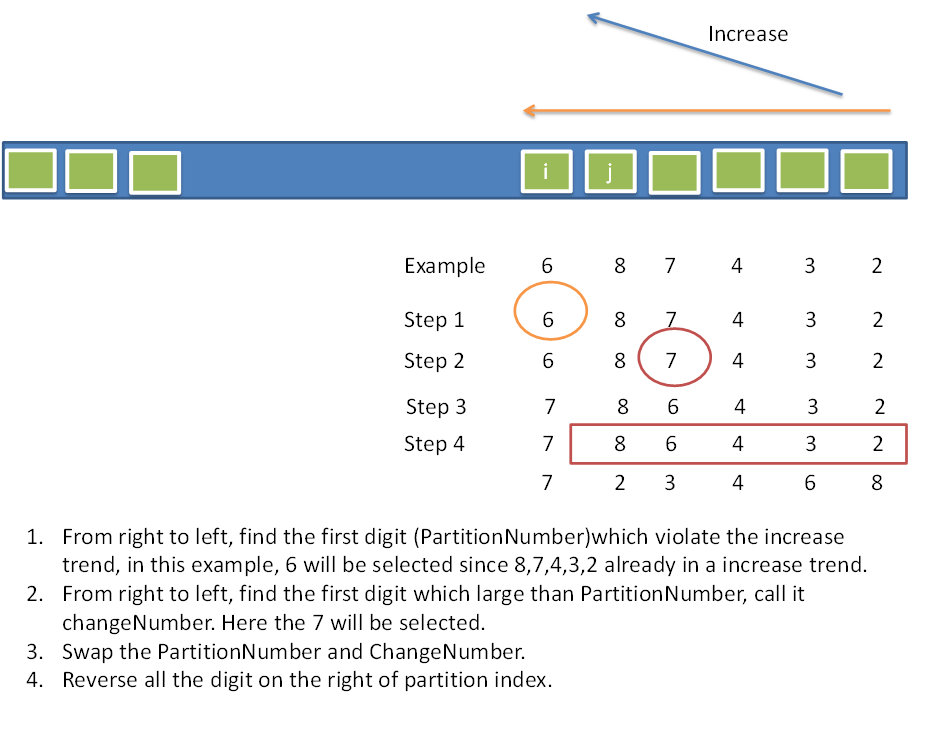
\includegraphics[width=360pt]{next-permutation.png}\\
\figcaption{下一个排列算法流程}\label{fig:permutation}
\end{center}


\subsubsection{代码}
\begin{Code}
// LintCode, Next Permutation
// 时间复杂度O(n),空间复杂度O(1)
class Solution {
    public:
    vector<int> nextPermutation(vector<int> &num) {
        vector<int> nums_copy(num);
        next_permutation(nums_copy.begin(), nums_copy.end());
        return nums_copy;
    }
    
    template<typename BidiIt>
    bool next_permutation(BidiIt first, BidiIt last) {
        // Get a reversed range to simplify reversed traversal.
        const auto rfirst = reverse_iterator<BidiIt>(last);
        const auto rlast = reverse_iterator<BidiIt>(first);
        
        // Begin from the second last element to the first element.
        auto pivot = next(rfirst);
        
        // Find `pivot`, which is the first element that is no less than its
        // successor.  `Prev` is used since `pivort` is a `reversed_iterator`.
        while (pivot != rlast && *pivot >= *prev(pivot))
        ++pivot;
        
        // No such elemenet found, current sequence is already the largest
        // permutation, then rearrange to the first permutation and return false.
        if (pivot == rlast) {
            reverse(rfirst, rlast);
            return false;
        }
        
        // Scan from right to left, find the first element that is greater than
        // `pivot`.
        auto change = find_if(rfirst, pivot, bind1st(less<int>(), *pivot));
        
        swap(*change, *pivot);
        reverse(rfirst, pivot);
        
        return true;
    }
};
\end{Code}


\subsubsection{相关题目}
\begindot
\item Permutation Sequence, 见 \S \ref{sec:permutation-sequence}
\item Permutations, 见 \S \ref{sec:permutations}
\item Permutations II, 见 \S \ref{sec:permutations-ii}
\item Combinations, 见 \S \ref{sec:combinations}
\myenddot


\subsection{Permutation Sequence} %%%%%%%%%%%%%%%%%%%%%%%%%%%%%%
\label{sec:permutation-sequence}


\subsubsection{描述}
The set \fn{[1,2,3,…,n]} contains a total of $n!$ unique permutations.

By listing and labeling all of the permutations in order,
We get the following sequence (ie, for $n = 3$):
\begin{Code}
"123"
"132"
"213"
"231"
"312"
"321"
\end{Code}

Given $n$ and $k$, return the kth permutation sequence.

Note: Given $n$ will be between 1 and 9 inclusive.


\subsubsection{分析}
简单的,可以用暴力枚举法,调用 $k-1$ 次 \fn{next_permutation()}。

暴力枚举法把前 $k$个排列都求出来了,比较浪费,而我们只需要第$k$个排列。

利用康托编码的思路,假设有$n$个不重复的元素,第$k$个排列是$a_1, a_2, a_3, ..., a_n$,那么$a_1$是哪一个位置呢?

我们把$a_1$去掉,那么剩下的排列为
$a_2, a_3, ..., a_n$, 共计$n-1$个元素,$n-1$个元素共有$(n-1)!$个排列,于是就可以知道 $a_1 = k / (n-1)!$。

同理,$a_2, a_3, ..., a_n$的值推导如下:

\begin{eqnarray}
k_2 &=& k\%(n-1)! \nonumber \\
a_2 &=& k_2/(n-2)! \nonumber \\
\quad & \cdots \nonumber \\
k_{n-1} &=& k_{n-2}\%2! \nonumber \\
a_{n-1} &=& k_{n-1}/1! \nonumber \\
a_n &=& 0 \nonumber
\end{eqnarray}


\subsubsection{使用next_permutation()}
\begin{Code}
// LintCode, Permutation Sequence
// 使用next_permutation(),TLE
class Solution {
public:
    string getPermutation(int n, int k) {
        string s(n, '0');
        for (int i = 0; i < n; ++i)
            s[i] += i+1;
        for (int i = 0; i < k-1; ++i)
            next_permutation(s.begin(), s.end());
        return s;
    }

    template<typename BidiIt>
    bool next_permutation(BidiIt first, BidiIt last) {
        // 代码见上一题 Next Permutation
    }
};
\end{Code}


\subsubsection{康托编码}
\begin{Code}
// LintCode, Permutation Sequence
// 康托编码,时间复杂度O(n),空间复杂度O(1)
class Solution {
public:
    string getPermutation(int n, int k) {
        string s(n, '0');
        string result;
        for (int i = 0; i < n; ++i)
            s[i] += i + 1;

        return kth_permutation(s, k);
    }
private:
    int factorial(int n) {
        int result = 1;
        for (int i = 1; i <= n; ++i)
            result *= i;
        return result;
    }

    // seq 已排好序,是第一个排列
    template<typename Sequence>
    Sequence kth_permutation(const Sequence &seq, int k) {
        const int n = seq.size();
        Sequence S(seq);
        Sequence result;

        int base = factorial(n - 1);
        --k;  // 康托编码从0开始

        for (int i = n - 1; i > 0; k %= base, base /= i, --i) {
            auto a = next(S.begin(), k / base);
            result.push_back(*a);
            S.erase(a);
        }

        result.push_back(S[0]); // 最后一个
        return result;
    }
};
\end{Code}


\subsubsection{相关题目}
\begindot
\item Next Permutation, 见 \S \ref{sec:next-permutation}
\item Permutations, 见 \S \ref{sec:permutations}
\item Permutations II, 见 \S \ref{sec:permutations-ii}
\item Combinations, 见 \S \ref{sec:combinations}
\myenddot


\subsection{Valid Sudoku} %%%%%%%%%%%%%%%%%%%%%%%%%%%%%%
\label{sec:valid-sudoku}


\subsubsection{描述}
Determine if a Sudoku is valid, according to: Sudoku Puzzles - The Rules \myurl{http://sudoku.com.au/TheRules.aspx} .

The Sudoku board could be partially filled, where empty cells are filled with the character \fn{'.'}.

\begin{center}
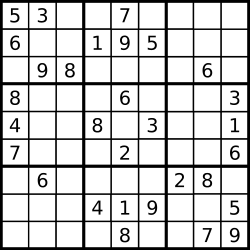
\includegraphics[width=150pt]{sudoku.png}\\
\figcaption{A partially filled sudoku which is valid}\label{fig:sudoku}
\end{center}

\subsubsection{分析}
细节实现题。


\subsubsection{代码}
\begin{Code}
// LintCode, Valid Sudoku
// 时间复杂度O(n^2),空间复杂度O(1)
class Solution {
public:
    bool isValidSudoku(const vector<vector<char>>& board) {
        bool used[9];

        for (int i = 0; i < 9; ++i) {
            fill(used, used + 9, false);

            for (int j = 0; j < 9; ++j) // 检查行
                if (!check(board[i][j], used))
                    return false;

            fill(used, used + 9, false);

            for (int j = 0; j < 9; ++j) // 检查列
                if (!check(board[j][i], used))
                    return false;
        }

        for (int r = 0; r < 3; ++r) // 检查 9 个子格子
            for (int c = 0; c < 3; ++c) {
                fill(used, used + 9, false);

                for (int i = r * 3; i < r * 3 + 3; ++i)
                    for (int j = c * 3; j < c * 3 + 3; ++j)
                        if (!check(board[i][j], used))
                            return false;
            }

        return true;
    }

    bool check(char ch, bool used[9]) {
        if (ch == '.') return true;

        if (used[ch - '1']) return false;

        return used[ch - '1'] = true;
    }
};
\end{Code}


\subsubsection{相关题目}
\begindot
\item Sudoku Solver, 见 \S \ref{sec:sudoku-solver}
\myenddot


\subsection{Trapping Rain Water} %%%%%%%%%%%%%%%%%%%%%%%%%%%%%%
\label{sec:trapping-rain-water}


\subsubsection{描述}
Given $n$ non-negative integers representing an elevation map where the width of each bar is 1, compute how much water it is able to trap after raining.

For example, 
Given \code{[0,1,0,2,1,0,1,3,2,1,2,1]}, return 6.

\begin{center}
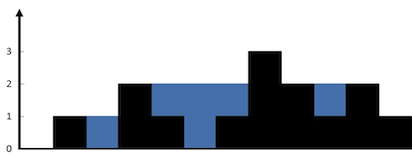
\includegraphics{trapping-rain-water.png}\\
\figcaption{Trapping Rain Water}\label{fig:trapping-rain-water}
\end{center}


\subsubsection{分析}
对于每个柱子,找到其左右两边最高的柱子,该柱子能容纳的面积就是\code{min(max_left, max_right) - height}。所以,
\begin{enumerate}
\item 从左往右扫描一遍,对于每个柱子,求取左边最大值;
\item 从右往左扫描一遍,对于每个柱子,求最大右值;
\item 再扫描一遍,把每个柱子的面积并累加。
\end{enumerate}

也可以,
\begin{enumerate}
\item 扫描一遍,找到最高的柱子,这个柱子将数组分为两半;
\item 处理左边一半;
\item 处理右边一半。
\end{enumerate}


\subsubsection{代码1}
\begin{Code}
// LintCode, Trapping Rain Water
// 思路1,时间复杂度O(n),空间复杂度O(n)
class Solution {
    public:
    int trapRainWater(const vector<int> &heights) {
        const int n = heights.size();
        auto max_left = vector<int>(n, 0);
        auto max_right = vector<int>(n, 0);
        
        for (int i = 1; i < n; i++) {
            max_left[i] = max(max_left[i - 1], heights[i - 1]);
            max_right[n - 1 - i] = max(max_right[n - i], heights[n - i]);
        }
        int sum = 0;
        for (int i = 0; i < n; i++) {
            int height = min(max_left[i], max_right[i]);
            if (height > heights[i]) {
                sum += height - heights[i];
            }
        }
        
        return sum;
    }
};
\end{Code}


\subsubsection{代码2}
\begin{Code}
// LintCode, Trapping Rain Water
// 思路2,时间复杂度O(n),空间复杂度O(1)
class Solution {
    public:
    int trapRainWater(const vector<int> &heights) {
        const int n = heights.size();
        int max = 0; // 最高的柱子,将数组分为两半
        for (int i = 0; i < n; i++)
        if (heights[i] > heights[max]) max = i;
        
        int water = 0;
        for (int i = 0, peak = 0; i < max; i++) {
            if (heights[i] > peak) peak = heights[i];
            else water += peak - heights[i];
        }
        for (int i = n - 1, top = 0; i > max; i--) {
            if (heights[i] > top) top = heights[i];
            else water += top - heights[i];
        }
        return water;
    }
};
\end{Code}


\subsubsection{代码3}
第三种解法,用一个栈辅助,小于栈顶的元素压入,大于等于栈顶就把栈里所有小于或等于当前值的元素全部出栈处理掉。
\begin{Code}
// LintCode, Trapping Rain Water
// 用一个栈辅助,小于栈顶的元素压入,大于等于栈顶就把栈里所有小于或
// 等于当前值的元素全部出栈处理掉,计算面积,最后把当前元素入栈
// 时间复杂度O(n),空间复杂度O(n)
class Solution {
    public:
    int trapRainWater(const vector<int> &heights) {
        const int n = heights.size();
        stack<pair<int, int>> s;
        int water = 0;
        
        for (int i = 0; i < n; ++i) {
            int height = 0;
            
            while (!s.empty()) { // 将栈里比当前元素矮或等高的元素全部处理掉
                int bar = s.top().first;
                int pos = s.top().second;
                // bar, height, a[i] 三者夹成的凹陷
                water += (min(bar, heights[i]) - height) * (i - pos - 1);
                height = bar;
                
                if (heights[i] < bar) // 碰到了比当前元素高的,跳出循环
                    break;
                else
                    s.pop(); // 弹出栈顶,因为该元素处理完了,不再需要了
            }
            
            s.push(make_pair(heights[i], i));
        }
        
        return water;
    }
};
\end{Code}


\subsubsection{相关题目}
\begindot
\item Container With Most Water, 见 \S \ref{sec:container-with-most-water}
\item Largest Rectangle in Histogram, 见 \S \ref{sec:largest-rectangle-in-histogram}
\myenddot


\subsection{Rotate Image} %%%%%%%%%%%%%%%%%%%%%%%%%%%%%%
\label{sec:rotate-image}


\subsubsection{描述}
You are given an $n \times n$ 2D matrix representing an image.

Rotate the image by 90 degrees (clockwise).

Follow up:
Could you do this in-place?


\subsubsection{分析}
首先想到,纯模拟,从外到内一圈一圈的转,但这个方法太慢。

如下图,首先沿着副对角线翻转一次,然后沿着水平中线翻转一次。

\begin{center}
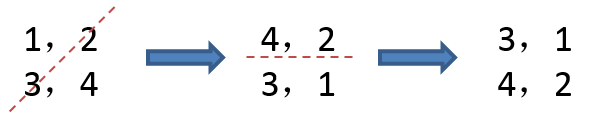
\includegraphics[width=200pt]{rotate-image.png}\\
\figcaption{Rotate Image}\label{fig:rotate-image}
\end{center}

或者,首先沿着水平中线翻转一次,然后沿着主对角线翻转一次。


\subsubsection{代码1}
\begin{Code}
// LintCode, Rotate Image
// 思路 1,时间复杂度O(n^2),空间复杂度O(1)
class Solution {
public:
    void rotate(vector<vector<int>>& matrix) {
        const int n = matrix.size();

        for (int i = 0; i < n; ++i)  // 沿着副对角线反转
            for (int j = 0; j < n - i; ++j)
                swap(matrix[i][j], matrix[n - 1 - j][n - 1 - i]);

        for (int i = 0; i < n / 2; ++i) // 沿着水平中线反转
            for (int j = 0; j < n; ++j)
                swap(matrix[i][j], matrix[n - 1 - i][j]);
    }
};
\end{Code}

\subsubsection{代码2}
\begin{Code}
// LintCode, Rotate Image
// 思路 2,时间复杂度O(n^2),空间复杂度O(1)
class Solution {
public:
    void rotate(vector<vector<int>>& matrix) {
        const int n = matrix.size();

        for (int i = 0; i < n / 2; ++i) // 沿着水平中线反转
            for (int j = 0; j < n; ++j)
                swap(matrix[i][j], matrix[n - 1 - i][j]);

        for (int i = 0; i < n; ++i)  // 沿着主对角线反转
            for (int j = i + 1; j < n; ++j)
                swap(matrix[i][j], matrix[j][i]);
    }
};
\end{Code}


\subsubsection{相关题目}
\begindot
\item 无
\myenddot


\subsection{Plus One} %%%%%%%%%%%%%%%%%%%%%%%%%%%%%%
\label{sec:plus-one}


\subsubsection{描述}
Given a number represented as an array of digits, plus one to the number.


\subsubsection{分析}
高精度加法。


\subsubsection{代码1}
\begin{Code}
// LintCode, Plus One
// 时间复杂度O(n),空间复杂度O(1)
class Solution {
public:
    vector<int> plusOne(vector<int> &digits) {
        add(digits, 1);
        return digits;
    }
private:
    // 0 <= digit <= 9
    void add(vector<int> &digits, int digit) {
        int c = digit;  // carry, 进位

        for (auto it = digits.rbegin(); it != digits.rend(); ++it) {
            *it += c;
            c = *it / 10;
            *it %= 10;
        }

        if (c > 0) digits.insert(digits.begin(), 1);
    }
};
\end{Code}


\subsubsection{代码2}
\begin{Code}
// LintCode, Plus One
// 时间复杂度O(n),空间复杂度O(1)
class Solution {
public:
    vector<int> plusOne(vector<int> &digits) {
        add(digits, 1);
        return digits;
    }
private:
    // 0 <= digit <= 9
    void add(vector<int> &digits, int digit) {
        int c = digit;  // carry, 进位

        for_each(digits.rbegin(), digits.rend(), [&c](int &d){
            d += c;
            c = d / 10;
            d %= 10;
        });

        if (c > 0) digits.insert(digits.begin(), 1);
    }
};
\end{Code}


\subsubsection{相关题目}
\begindot
\item 无
\myenddot


\subsection{Climbing Stairs} %%%%%%%%%%%%%%%%%%%%%%%%%%%%%%
\label{sec:climbing-stairs}


\subsubsection{描述}
You are climbing a stair case. It takes $n$ steps to reach to the top.

Each time you can either climb 1 or 2 steps. In how many distinct ways can you climb to the top?


\subsubsection{分析}
设$f(n)$表示爬$n$阶楼梯的不同方法数,为了爬到第$n$阶楼梯,有两个选择:
\begindot
\item 从第$n-1$阶前进1步;
\item 从第$n-1$阶前进2步;
\myenddot
因此,有$f(n)=f(n-1)+f(n-2)$。

这是一个斐波那契数列。

方法1,递归,太慢;方法2,迭代。

方法3,数学公式。斐波那契数列的通项公式为 $a_n=\dfrac{1}{\sqrt{5}}\left[\left(\dfrac{1+\sqrt{5}}{2}\right)^n-\left(\dfrac{1-\sqrt{5}}{2}\right)^n\right]$。


\subsubsection{迭代}
\begin{Code}
// LintCode, Climbing Stairs
// 迭代,时间复杂度O(n),空间复杂度O(1)
class Solution {
public:
    int climbStairs(int n) {
        int prev = 0;
        int cur = 1;
        for(int i = 1; i <= n ; ++i){
            int tmp = cur;
            cur += prev;
            prev = tmp;
        }
        return cur;
    }
};
\end{Code}


\subsubsection{数学公式}
\begin{Code}
// LintCode, Climbing Stairs
// 数学公式,时间复杂度O(1),空间复杂度O(1)
class Solution {
    public:
    int climbStairs(int n) {
        const double s = sqrt(5);
        return floor((pow((1+s)/2, n+1) + pow((1-s)/2, n+1))/s + 0.5);
    }
};
\end{Code}


\subsubsection{相关题目}
\begindot
\item Decode Ways, 见 \S \ref{sec:decode-ways}
\myenddot


\subsection{Gray Code} %%%%%%%%%%%%%%%%%%%%%%%%%%%%%%
\label{sec:gray-code}


\subsubsection{描述}
The gray code is a binary numeral system where two successive values differ in only one bit.

Given a non-negative integer $n$ representing the total number of bits in the code, print the sequence of gray code. A gray code sequence must begin with 0.

For example, given $n = 2$, return \fn{[0,1,3,2]}. Its gray code sequence is:
\begin{Code}
00 - 0
01 - 1
11 - 3
10 - 2
\end{Code}

Note:
\begindot
\item For a given $n$, a gray code sequence is not uniquely defined.
\item For example, \fn{[0,2,3,1]} is also a valid gray code sequence according to the above definition.
\item For now, the judge is able to judge based on one instance of gray code sequence. Sorry about that.
\myenddot


\subsubsection{分析}
格雷码(Gray Code)的定义请参考 \myurl{http://en.wikipedia.org/wiki/Gray_code}

\textbf{自然二进制码转换为格雷码:$g_0=b_0, g_i=b_i \oplus b_{i-1}$}

保留自然二进制码的最高位作为格雷码的最高位,格雷码次高位为二进制码的高位与次高位异或,其余各位与次高位的求法类似。例如,将自然二进制码1001,转换为格雷码的过程是:保留最高位;然后将第1位的1和第2位的0异或,得到1,作为格雷码的第2位;将第2位的0和第3位的0异或,得到0,作为格雷码的第3位;将第3位的0和第4位的1异或,得到1,作为格雷码的第4位,最终,格雷码为1101。

\textbf{格雷码转换为自然二进制码:$b_0=g_0, b_i=g_i \oplus b_{i-1}$}

保留格雷码的最高位作为自然二进制码的最高位,次高位为自然二进制高位与格雷码次高位异或,其余各位与次高位的求法类似。例如,将格雷码1000转换为自然二进制码的过程是:保留最高位1,作为自然二进制码的最高位;然后将自然二进制码的第1位1和格雷码的第2位0异或,得到1,作为自然二进制码的第2位;将自然二进制码的第2位1和格雷码的第3位0异或,得到1,作为自然二进制码的第3位;将自然二进制码的第3位1和格雷码的第4位0异或,得到1,作为自然二进制码的第4位,最终,自然二进制码为1111。

格雷码有\textbf{数学公式},整数$n$的格雷码是$n \oplus (n/2)$。

这题要求生成$n$比特的所有格雷码。

方法1,最简单的方法,利用数学公式,对从 $0\sim2^n-1$的所有整数,转化为格雷码。

方法2,$n$比特的格雷码,可以递归地从$n-1$比特的格雷码生成。如图\S \ref{fig:gray-code-construction}所示。

\begin{center}
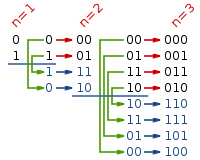
\includegraphics[width=160pt]{gray-code-construction.png}\\
\figcaption{The first few steps of the reflect-and-prefix method.}\label{fig:gray-code-construction}
\end{center}


\subsubsection{数学公式}
\begin{Code}
// LintCode, Gray Code
// 数学公式,时间复杂度O(2^n),空间复杂度O(1)
class Solution {
public:
    vector<int> grayCode(int n) {
        vector<int> result;
        const size_t size = 1 << n;  // 2^n
        result.reserve(size);
        for (size_t i = 0; i < size; ++i)
            result.push_back(binary_to_gray(i));
        return result;
    }
private:
    static unsigned int binary_to_gray(unsigned int n) {
        return n ^ (n >> 1);
    }
};
\end{Code}


\subsubsection{Reflect-and-prefix method}
\begin{Code}
// LintCode, Gray Code
// reflect-and-prefix method
// 时间复杂度O(2^n),空间复杂度O(1)
class Solution {
public:
    vector<int> grayCode(int n) {
        vector<int> result;
        result.reserve(1<<n);
        result.push_back(0);
        for (int i = 0; i < n; i++) {
            const int highest_bit = 1 << i;
            for (int j = result.size() - 1; j >= 0; j--) // 要反着遍历,才能对称
                result.push_back(highest_bit | result[j]);
        }
        return result;
    }
};
\end{Code}


\subsubsection{相关题目}
\begindot
\item 无
\myenddot


\subsection{Set Matrix Zeroes} %%%%%%%%%%%%%%%%%%%%%%%%%%%%%%
\label{sec:set-matrix-zeroes}


\subsubsection{描述}
Given a $m \times n$ matrix, if an element is 0, set its entire row and column to 0. Do it in place.

\textbf{Follow up:}
Did you use extra space?

A straight forward solution using $O(mn)$ space is probably a bad idea.

A simple improvement uses $O(m + n)$ space, but still not the best solution.

Could you devise a constant space solution?


\subsubsection{分析}
$O(m+n)$空间的方法很简单,设置两个bool数组,记录每行和每列是否存在0。

想要常数空间,可以复用第一行和第一列。


\subsubsection{代码1}
\begin{Code}
// LintCode, Set Matrix Zeroes
// 时间复杂度O(m*n),空间复杂度O(m+n)
class Solution {
    public:
    void setZeroes(vector<vector<int> > &matrix) {
        const size_t m = matrix.size();
        if (m == 0) return;
        const size_t n = matrix[0].size();
        
        vector<bool> row(m, false); // 标记该行是否存在0
        vector<bool> col(n, false); // 标记该列是否存在0
        
        for (size_t i = 0; i < m; ++i) {
            for (size_t j = 0; j < n; ++j) {
                if (matrix[i][j] == 0) {
                    row[i] = col[j] = true;
                }
            }
        }
        for (size_t i = 0; i < m; ++i) {
            if (row[i])
            fill(&matrix[i][0], &matrix[i][0] + n, 0);
        }
        for (size_t j = 0; j < n; ++j) {
            if (col[j]) {
                for (size_t i = 0; i < m; ++i) {
                    matrix[i][j] = 0;
                }
            }
        }
    }
};
\end{Code}


\subsubsection{代码2}
\begin{Code}
// LintCode, Set Matrix Zeroes
// 时间复杂度O(m*n),空间复杂度O(1)
class Solution {
    public:
    void setZeroes(vector<vector<int> > &matrix) {
        const size_t m = matrix.size();
        if (m == 0) return;
        const size_t n = matrix[0].size();
        bool row_has_zero = false; // 第一行是否存在 0
        bool col_has_zero = false; // 第一列是否存在 0
        
        for (size_t i = 0; i < n; i++)
        if (matrix[0][i] == 0) {
            row_has_zero = true;
            break;
        }
        
        for (size_t i = 0; i < m; i++)
        if (matrix[i][0] == 0) {
            col_has_zero = true;
            break;
        }
        
        for (size_t i = 1; i < m; i++)
        for (size_t j = 1; j < n; j++)
        if (matrix[i][j] == 0) {
            matrix[0][j] = 0;
            matrix[i][0] = 0;
        }
        for (size_t i = 1; i < m; i++)
        for (size_t j = 1; j < n; j++)
        if (matrix[i][0] == 0 || matrix[0][j] == 0)
        matrix[i][j] = 0;
        if (row_has_zero)
        for (size_t i = 0; i < n; i++)
        matrix[0][i] = 0;
        if (col_has_zero)
        for (size_t i = 0; i < m; i++)
        matrix[i][0] = 0;
    }
};
\end{Code}


\subsubsection{相关题目}
\begindot
\item 无
\myenddot


\subsection{Gas Station} %%%%%%%%%%%%%%%%%%%%%%%%%%%%%%
\label{sec:gas-station}


\subsubsection{描述}
There are $N$ gas stations along a circular route, where the amount of gas at station $i$ is \fn{gas[i]}.

You have a car with an unlimited gas tank and it costs \fn{cost[i]} of gas to travel from station $i$ to its next station ($i$+1). You begin the journey with an empty tank at one of the gas stations.

Return the starting gas station's index if you can travel around the circuit once, otherwise return -1.

Note:
The solution is guaranteed to be unique.


\subsubsection{分析}
首先想到的是$O(N^2)$的解法,对每个点进行模拟。

$O(N)$的解法是,设置两个变量,\fn{sum}判断当前的指针的有效性;\fn{total}则判断整个数组是否有解,有就返回通过\fn{sum}得到的下标,没有则返回-1。


\subsubsection{代码}
\begin{Code}
// LintCode, Gas Station
// 时间复杂度O(n),空间复杂度O(1)
class Solution {
public:
    int canCompleteCircuit(vector<int> &gas, vector<int> &cost) {
        int total = 0;
        int j = -1;
        for (int i = 0, sum = 0; i < gas.size(); ++i) {
            sum += gas[i] - cost[i];
            total += gas[i] - cost[i];
            if (sum < 0) {
                j = i;
                sum = 0;
            }
        }
        return total >= 0 ? j + 1 : -1;
    }
};
\end{Code}


\subsubsection{相关题目}
\begindot
\item 无
\myenddot


\subsection{Candy} %%%%%%%%%%%%%%%%%%%%%%%%%%%%%%
\label{sec:candy}


\subsubsection{描述}
There are $N$ children standing in a line. Each child is assigned a rating value.

You are giving candies to these children subjected to the following requirements:
\begindot
\item Each child must have at least one candy.
\item Children with a higher rating get more candies than their neighbors.
\myenddot

What is the minimum candies you must give?


\subsubsection{分析}
无


\subsubsection{迭代版}
\begin{Code}
// LintCode, Candy
// 时间复杂度O(n),空间复杂度O(n)
class Solution {
public:
    int candy(vector<int> &ratings) {
        const int n = ratings.size();
        vector<int> increment(n);

        // 左右各扫描一遍
        for (int i = 1, inc = 1; i < n; i++) {
            if (ratings[i] > ratings[i - 1])
                increment[i] = max(inc++, increment[i]);
            else
                inc = 1;
        }

        for (int i = n - 2, inc = 1; i >= 0; i--) {
            if (ratings[i] > ratings[i + 1])
                increment[i] = max(inc++, increment[i]);
            else
                inc = 1;
        }
        // 初始值为n,因为每个小朋友至少一颗糖
        return accumulate(&increment[0], &increment[0]+n, n);
    }
};
\end{Code}


\subsubsection{递归版}
\begin{Code}
// LintCode, Candy
// 备忘录法,时间复杂度O(n),空间复杂度O(n)
// @author fancymouse (http://weibo.com/u/1928162822)
class Solution {
public:
    int candy(const vector<int>& ratings) {
        vector<int> f(ratings.size());
        int sum = 0;
        for (int i = 0; i < ratings.size(); ++i)
            sum += solve(ratings, f, i);
        return sum;
    }
    int solve(const vector<int>& ratings, vector<int>& f, int i) {
        if (f[i] == 0) {
            f[i] = 1;
            if (i > 0 && ratings[i] > ratings[i - 1])
                f[i] = max(f[i], solve(ratings, f, i - 1) + 1);
            if (i < ratings.size() - 1 && ratings[i] > ratings[i + 1])
                f[i] = max(f[i], solve(ratings, f, i + 1) + 1);
        }
        return f[i];
    }
};
\end{Code}


\subsubsection{相关题目}
\begindot
\item 无
\myenddot


\subsection{Single Number} %%%%%%%%%%%%%%%%%%%%%%%%%%%%%%
\label{sec:single-number}


\subsubsection{描述}
Given an array of integers, every element appears twice except for one. Find that single one.

Note:
Your algorithm should have a linear runtime complexity. Could you implement it without using extra memory?


\subsubsection{分析}
异或,不仅能处理两次的情况,只要出现偶数次,都可以清零。


\subsubsection{代码1}
\begin{Code}
// LintCode, Single Number
// 时间复杂度O(n),空间复杂度O(1)
class Solution {
    public:
    int singleNumber(const vector<int> &A) {
        int x = 0;
        for (auto i : A) {
            x ^= i;
        }
        return x;
    }
};
\end{Code}


\subsubsection{代码2}
\begin{Code}
// LintCode, Single Number
// 时间复杂度O(n),空间复杂度O(1)
class Solution {
    public:
    int singleNumber(const vector<int> &A) {
        return accumulate(A.begin(), A.end(), 0, bit_xor<int>());
    }
};
\end{Code}


\subsubsection{相关题目}
\begindot
\item  Single Number II, 见 \S \ref{sec:single-number-ii}
\myenddot


\subsection{Single Number II} %%%%%%%%%%%%%%%%%%%%%%%%%%%%%%
\label{sec:single-number-ii}


\subsubsection{描述}
Given an array of integers, every element appears three times except for one. Find that single one.

Note:
Your algorithm should have a linear runtime complexity. Could you implement it without using extra memory?


\subsubsection{分析}
本题和上一题 Single Number,考察的是位运算。

方法1:创建一个长度为\fn{sizeof(int)}的数组\fn{count[sizeof(int)]},\fn{count[i]}表示在在$i$位出现的1的次数。如果\fn{count[i]}是3的整数倍,则忽略;否则就把该位取出来组成答案。

方法2:用\fn{one}记录到当前处理的元素为止,二进制1出现“1次”(mod 3 之后的 1)的有哪些二进制位;用\fn{two}记录到当前计算的变量为止,二进制1出现“2次”(mod 3 之后的 2)的有哪些二进制位。当\fn{one}和\fn{two}中的某一位同时为1时表示该二进制位上1出现了3次,此时需要清零。即\textbf{用二进制模拟三进制运算}。最终\fn{one}记录的是最终结果。

\subsubsection{代码1}
\begin{Code}
// LintCode, Single Number II
// 方法1,时间复杂度O(n),空间复杂度O(1)
class Solution {
    public:
    int singleNumberII(const vector<int> &A) {
        const int W = sizeof(int) * 8; // 一个整数的bit数,即整数字长
        int count[W];  // count[i]表示在在i位出现的1的次数
        fill_n(&count[0], W, 0);
        for (int i = 0; i < A.size(); i++) {
            for (int j = 0; j < W; j++) {
                count[j] += (A[i] >> j) & 1;
                count[j] %= 3;
            }
        }
        int result = 0;
        for (int i = 0; i < W; i++) {
            result += (count[i] << i);
        }
        return result;
    }
};
\end{Code}


\subsubsection{代码2}
\begin{Code}
// LintCode, Single Number II
// 方法2,时间复杂度O(n),空间复杂度O(1)
class Solution {
    public:
    int singleNumberII(const vector<int> &A) {
        int one = 0, two = 0, three = 0;
        for (int i = 0; i < A.size(); ++i) {
            two |= (one & A[i]);
            one ^= A[i];
            three = ~(one & two);
            one &= three;
            two &= three;
        }
        
        return one;
    }
};
\end{Code}


\subsubsection{相关题目}
\begindot
\item  Single Number, 见 \S \ref{sec:single-number}
\myenddot


\section{单链表} %%%%%%%%%%%%%%%%%%%%%%%%%%%%%%

单链表节点的定义如下:
\begin{Code}
// 单链表节点
struct ListNode {
    int val;
    ListNode *next;
    ListNode(int x) : val(x), next(nullptr) { }
};
\end{Code}


\subsection{Add Two Numbers}
\label{sec:add-two-numbers}


\subsubsection{描述}
You are given two linked lists representing two non-negative numbers. The digits are stored in reverse order and each of their nodes contain a single digit. Add the two numbers and return it as a linked list.

Input: {\small \fontspec{Latin Modern Mono} (2 -> 4 -> 3) + (5 -> 6 -> 4)}

Output: {\small \fontspec{Latin Modern Mono} 7 -> 0 -> 8}


\subsubsection{分析}
跟Add Binary(见 \S \ref{sec:add-binary})很类似


\subsubsection{代码}
\begin{Code}
// LintCode, Add Two Numbers
// 跟Add Binary 很类似
// 时间复杂度O(m+n),空间复杂度O(1)
class Solution {
public:
    ListNode *addTwoNumbers(ListNode *l1, ListNode *l2) {
        ListNode dummy(-1); // 头节点
        int carry = 0;
        ListNode *prev = &dummy;
        for (ListNode *pa = l1, *pb = l2;
             pa != nullptr || pb != nullptr;
             pa = pa == nullptr ? nullptr : pa->next,
             pb = pb == nullptr ? nullptr : pb->next,
             prev = prev->next) {
            const int ai = pa == nullptr ? 0 : pa->val;
            const int bi = pb == nullptr ? 0 : pb->val;
            const int value = (ai + bi + carry) % 10;
            carry = (ai + bi + carry) / 10;
            prev->next = new ListNode(value); // 尾插法
        }
        if (carry > 0)
            prev->next = new ListNode(carry);
        return dummy.next;
    }
};
\end{Code}


\subsubsection{相关题目}

\begindot
\item Add Binary, 见 \S \ref{sec:add-binary}
\myenddot


\subsection{Reverse Linked List}
\label{sec:reverse-linked-list}


\subsubsection{描述}
Reverse a single linked list.

Example:
Given a linked list
For linked list \code{1->2->3->nullptr}, return \code{3->2->1->nullptr}.


\subsubsection{分析}
这是一道很基本的单链表题目,考察你对单链表的理解程度。


\subsubsection{递归版}
\begin{Code}
class Solution {
    public:
    ListNode* reverse(ListNode *head) {
        if (head == nullptr || head->next == nullptr) return head;
        ListNode* tail = head->next;
        ListNode *head_of_reversed_tail = reverse(tail);
        tail->next = head;
        head->next = nullptr;
        return head_of_reversed_tail;
    }
};
\end{Code}


\subsubsection{迭代版}
\begin{Code}
class Solution {
public:
    ListNode* reverse(ListNode* head) {
        ListNode* prev = nullptr;
        while (head) {
            ListNode* next = head->next;
            head->next = prev;
            prev = head;
            head = next;
        }
        return prev;
    }
};
\end{Code}


\subsubsection{相关题目}

\begindot
\item Reverse Linked List II, 见 \S \ref{sec:reverse-linked-list-ii}
\myenddot


\subsection{Reverse Linked List II}
\label{sec:reverse-linked-list-ii}


\subsubsection{描述}
Reverse a linked list from position $m$ to $n$. Do it in-place and in one-pass.

For example:
Given \code{1->2->3->4->5->nullptr}, $m$ = 2 and $n$ = 4,

return \code{1->4->3->2->5->nullptr}.

Note:
Given m, n satisfy the following condition:
$1 \leq m \leq  n \leq $ length of list.


\subsubsection{分析}
这题非常繁琐,有很多边界检查,15分钟内做到bug free很有难度!


\subsubsection{代码}
\begin{Code}
// LintCode, Reverse Linked List II
// 迭代版,时间复杂度O(n),空间复杂度O(1)
class Solution {
public:
    ListNode *reverseBetween(ListNode *head, int m, int n) {
        ListNode dummy(-1);
        dummy.next = head;

        ListNode *prev = &dummy;
        for (int i = 0; i < m-1; ++i)
            prev = prev->next;
        ListNode* const head2 = prev;

        prev = head2->next;
        ListNode *cur = prev->next;
        for (int i = m; i < n; ++i) {
            prev->next = cur->next;
            cur->next = head2->next;
            head2->next = cur;  // 头插法
            cur = prev->next;
        }

        return dummy.next;
    }
};
\end{Code}


\subsubsection{相关题目}

\begindot
\item Reverse Linked List, 见 \S \ref{sec:reverse-linked-list}
\myenddot


\subsection{Partition List}
\label{sec:partition-list}


\subsubsection{描述}
Given a linked list and a value $x$, partition it such that all nodes less than $x$ come before nodes greater than or equal to $x$.

You should preserve the original relative order of the nodes in each of the two partitions.

For example,
Given \code{1->4->3->2->5->2} and \code{x = 3}, return \code{1->2->2->4->3->5}.


\subsubsection{分析}
无


\subsubsection{代码}
\begin{Code}
// LintCode, Partition List
// 时间复杂度O(n),空间复杂度O(1)
class Solution {
public:
    ListNode* partition(ListNode* head, int x) {
        ListNode left_dummy(-1); // 头结点
        ListNode right_dummy(-1); // 头结点

        auto left_cur = &left_dummy;
        auto right_cur = &right_dummy;

        for (ListNode *cur = head; cur; cur = cur->next) {
            if (cur->val < x) {
                left_cur->next = cur;
                left_cur = cur;
            } else {
                right_cur->next = cur;
                right_cur = cur;
            }
        }

        left_cur->next = right_dummy.next;
        right_cur->next = nullptr;

        return left_dummy.next;
    }
};
\end{Code}


\subsubsection{相关题目}

\begindot
\item 无
\myenddot


\subsection{Remove Duplicates from Sorted List}
\label{sec:remove-duplicates-from-sorted-list}


\subsubsection{描述}
Given a sorted linked list, delete all duplicates such that each element appear only once.

For example,

Given \code{1->1->2}, return \code{1->2}.

Given \code{1->1->2->3->3}, return \code{1->2->3}.


\subsubsection{分析}
无


\subsubsection{递归版}
\begin{Code}
// LintCode, Remove Duplicates from Sorted List
// 递归版,时间复杂度O(n),空间复杂度O(1)
class Solution {
public:
    ListNode *deleteDuplicates(ListNode *head) {
        if (!head) return head;
        ListNode dummy(head->val + 1); // 值只要跟head不同即可
        dummy.next = head;

        recur(&dummy, head);
        return dummy.next;
    }
private:
    static void recur(ListNode *prev, ListNode *cur) {
        if (cur == nullptr) return;

        if (prev->val == cur->val) { // 删除head
            prev->next = cur->next;
            delete cur;
            recur(prev, prev->next);
        } else {
            recur(prev->next, cur->next);
        }
    }
};
\end{Code}


\subsubsection{迭代版}
\begin{Code}
// LintCode, Remove Duplicates from Sorted List
// 迭代版,时间复杂度O(n),空间复杂度O(1)
class Solution {
public:
    ListNode *deleteDuplicates(ListNode *head) {
        if (head == nullptr) return nullptr;

        for (ListNode *prev = head, *cur = head->next; cur; cur = cur->next) {
            if (prev->val == cur->val) {
                prev->next = cur->next;
                delete cur;
            } else {
                prev = cur;
            }
        }
        return head;
    }
};
\end{Code}


\subsubsection{相关题目}

\begindot
\item Remove Duplicates from Sorted List II,见 \S \ref{sec:remove-duplicates-from-sorted-list-ii}
\myenddot


\subsection{Remove Duplicates from Sorted List II}
\label{sec:remove-duplicates-from-sorted-list-ii}


\subsubsection{描述}
Given a sorted linked list, delete all nodes that have duplicate numbers, leaving only distinct numbers from the original list.

For example,

Given \code{1->2->3->3->4->4->5}, return \code{1->2->5}.

Given \code{1->1->1->2->3}, return \code{2->3}.


\subsubsection{分析}
无


\subsubsection{递归版}
\begin{Code}
// LintCode, Remove Duplicates from Sorted List II
// 递归版,时间复杂度O(n),空间复杂度O(1)
class Solution {
public:
    ListNode *deleteDuplicates(ListNode *head) {
        if (!head || !head->next) return head;

        ListNode *p = head->next;
        if (head->val == p->val) {
            while (p && head->val == p->val) {
                ListNode *tmp = p;
                p = p->next;
                delete tmp;
            }
            delete head;
            return deleteDuplicates(p);
        } else {
            head->next = deleteDuplicates(head->next);
            return head;
        }
    }
};
\end{Code}


\subsubsection{迭代版}
\begin{Code}
// LintCode, Remove Duplicates from Sorted List II
// 迭代版,时间复杂度O(n),空间复杂度O(1)
class Solution {
public:
    ListNode *deleteDuplicates(ListNode *head) {
        if (head == nullptr) return head;

        ListNode dummy(INT_MIN); // 头结点
        dummy.next = head;
        ListNode *prev = &dummy, *cur = head;
        while (cur != nullptr) {
            bool duplicated = false;
            while (cur->next != nullptr && cur->val == cur->next->val) {
                duplicated = true;
                ListNode *temp = cur;
                cur = cur->next;
                delete temp;
            }
            if (duplicated) { // 删除重复的最后一个元素
                ListNode *temp = cur;
                cur = cur->next;
                delete temp;
                continue;
            }
            prev->next = cur;
            prev = prev->next;
            cur = cur->next;
        }
        prev->next = cur;
        return dummy.next;
    }
};
\end{Code}


\subsubsection{相关题目}

\begindot
\item Remove Duplicates from Sorted List,见 \S \ref{sec:remove-duplicates-from-sorted-list}
\myenddot


\subsection{Rotate List}
\label{sec:rotate-list}


\subsubsection{描述}
Given a list, rotate the list to the right by $k$ places, where $k$ is non-negative.

For example:
Given \code{1->2->3->4->5->nullptr} and \code{k = 2}, return \code{4->5->1->2->3->nullptr}.


\subsubsection{分析}
先遍历一遍,得出链表长度$len$,注意$k$可能大于$len$,因此令$k \%= len$。将尾节点next指针指向首节点,形成一个环,接着往后跑$len-k$步,从这里断开,就是要求的结果了。


\subsubsection{代码}
\begin{Code}
// LintCode, Remove Rotate List
// 时间复杂度O(n),空间复杂度O(1)
class Solution {
public:
    ListNode *rotateRight(ListNode *head, int k) {
        if (head == nullptr || k == 0) return head;

        int len = 1;
        ListNode* p = head;
        while (p->next) { // 求长度
            len++;
            p = p->next;
        }
        k = len - k % len;

        p->next = head; // 首尾相连
        for(int step = 0; step < k; step++) {
            p = p->next;  //接着往后跑
        }
        head = p->next; // 新的首节点
        p->next = nullptr; // 断开环
        return head;
    }
};
\end{Code}


\subsubsection{相关题目}

\begindot
\item 无
\myenddot


\subsection{Remove Nth Node From End of List}
\label{sec:remove-nth-node-from-end-of-list}


\subsubsection{描述}
Given a linked list, remove the $n^{th}$ node from the end of list and return its head.

For example, Given linked list: \code{1->2->3->4->5}, and $n$ = 2.

After removing the second node from the end, the linked list becomes \code{1->2->3->5}.

Note:
\begindot
\item Given $n$ will always be valid.
\item Try to do this in one pass.
\myenddot


\subsubsection{分析}
设两个指针$p,q$,让$q$先走$n$步,然后$p$和$q$一起走,直到$q$走到尾节点,删除\fn{p->next}即可。


\subsubsection{代码}
\begin{Code}
// LintCode, Remove Nth Node From End of List
// 时间复杂度O(n),空间复杂度O(1)
class Solution {
public:
    ListNode *removeNthFromEnd(ListNode *head, int n) {
        ListNode dummy{-1, head};
        ListNode *p = &dummy, *q = &dummy;

        for (int i = 0; i < n; i++)  // q先走n步
            q = q->next;

        while(q->next) { // 一起走
            p = p->next;
            q = q->next;
        }
        ListNode *tmp = p->next;
        p->next = p->next->next;
        delete tmp;
        return dummy.next;
    }
};
\end{Code}


\subsubsection{相关题目}

\begindot
\item 无
\myenddot


\subsection{Swap Nodes in Pairs}
\label{sec:swap-nodes-in-pairs}


\subsubsection{描述}
Given a linked list, swap every two adjacent nodes and return its head.

For example,
Given \code{1->2->3->4}, you should return the list as \code{2->1->4->3}.

Your algorithm should use only constant space. You may \emph{not} modify the values in the list, only nodes itself can be changed.


\subsubsection{分析}
无


\subsubsection{代码}
\begin{Code}
// LintCode, Swap Nodes in Pairs
// 时间复杂度O(n),空间复杂度O(1)
class Solution {
public:
    ListNode *swapPairs(ListNode *head) {
        if (head == nullptr || head->next == nullptr) return head;
        ListNode dummy(-1);
        dummy.next = head;

        for(ListNode *prev = &dummy, *cur = prev->next, *next = cur->next;
                next;
                prev = cur, cur = cur->next, next = cur ? cur->next: nullptr) {
            prev->next = next;
            cur->next = next->next;
            next->next = cur;
        }
        return dummy.next;
    }
};
\end{Code}

下面这种写法更简洁,但题目规定了不准这样做。
\begin{Code}
// LintCode, Swap Nodes in Pairs
// 时间复杂度O(n),空间复杂度O(1)
class Solution {
public:
    ListNode* swapPairs(ListNode* head) {
        ListNode* p = head;

        while (p && p->next) {
            swap(p->val, p->next->val);
            p = p->next->next;
        }

        return head;
    }
};
\end{Code}

\subsubsection{相关题目}

\begindot
\item Reverse Nodes in k-Group, 见 \S \ref{sec:reverse-nodes-in-k-group}
\myenddot


\subsection{Reverse Nodes in k-Group}
\label{sec:reverse-nodes-in-k-group}


\subsubsection{描述}
Given a linked list, reverse the nodes of a linked list k at a time and return its modified list.

If the number of nodes is not a multiple of $k$ then left-out nodes in the end should remain as it is.

You may not alter the values in the nodes, only nodes itself may be changed.

Only constant memory is allowed.

For example,
Given this linked list: \code{1->2->3->4->5}

For $k = 2$, you should return: \code{2->1->4->3->5}

For $k = 3$, you should return: \code{3->2->1->4->5}


\subsubsection{分析}
无


\subsubsection{递归版}
\begin{Code}
// LintCode, Reverse Nodes in k-Group
// 递归版,时间复杂度O(n),空间复杂度O(1)
class Solution {
public:
    ListNode *reverseKGroup(ListNode *head, int k) {
        if (head == nullptr || head->next == nullptr || k < 2)
            return head;

        ListNode *next_group = head;
        for (int i = 0; i < k; ++i) {
            if (next_group)
                next_group = next_group->next;
            else
                return head;
        }
        // next_group is the head of next group
        // new_next_group is the new head of next group after reversion
        ListNode *new_next_group = reverseKGroup(next_group, k);
        ListNode *prev = NULL, *cur = head;
        while (cur != next_group) {
            ListNode *next = cur->next;
            cur->next = prev ? prev : new_next_group;
            prev = cur;
            cur = next;
        }
        return prev; // prev will be the new head of this group
    }
};
\end{Code}


\subsubsection{迭代版}
\begin{Code}
// LintCode, Reverse Nodes in k-Group
// 迭代版,时间复杂度O(n),空间复杂度O(1)
class Solution {
public:
    ListNode *reverseKGroup(ListNode *head, int k) {
        if (head == nullptr || head->next == nullptr || k < 2) return head;
        ListNode dummy(-1);
        dummy.next = head;

        for(ListNode *prev = &dummy, *end = head; end; end = prev->next) {
            for (int i = 1; i < k && end; i++)
                end = end->next;
            if (end  == nullptr) break;  // 不足 k 个

            prev = reverse(prev, prev->next, end);
        }

        return dummy.next;
    }

    // prev 是 first 前一个元素, [begin, end] 闭区间,保证三者都不为 null
    // 返回反转后的倒数第1个元素
    ListNode* reverse(ListNode *prev, ListNode *begin, ListNode *end) {
        ListNode *end_next = end->next;
        for (ListNode *p = begin, *cur = p->next, *next = cur->next;
                cur != end_next;
                p = cur, cur = next, next = next ? next->next : nullptr) {
            cur->next = p;
        }
        begin->next = end_next;
        prev->next = end;
        return begin;
    }
};
\end{Code}


\subsubsection{相关题目}
\begindot
\item Swap Nodes in Pairs, 见 \S \ref{sec:swap-nodes-in-pairs}
\myenddot


\subsection{Copy List with Random Pointer}
\label{sec:copy-list-with-random-pointer}


\subsubsection{描述}
A linked list is given such that each node contains an additional random pointer which could point to any node in the list or null.

Return a deep copy of the list.


\subsubsection{分析}
无


\subsubsection{代码}
\begin{Code}
// LintCode, Copy List with Random Pointer
// 两遍扫描,时间复杂度O(n),空间复杂度O(1)
class Solution {
public:
    RandomListNode *copyRandomList(RandomListNode *head) {
        for (RandomListNode* cur = head; cur != nullptr; ) {
            RandomListNode* node = new RandomListNode(cur->label);
            node->next = cur->next;
            cur->next = node;
            cur = node->next;
        }

        for (RandomListNode* cur = head; cur != nullptr; ) {
            if (cur->random != NULL)
                cur->next->random = cur->random->next;
            cur = cur->next->next;
        }

        // 分拆两个单链表
        RandomListNode dummy(-1);
        for (RandomListNode* cur = head, *new_cur = &dummy;
                cur != nullptr; ) {
            new_cur->next = cur->next;
            new_cur = new_cur->next;
            cur->next = cur->next->next;
            cur = cur->next;
        }
        return dummy.next;
    }
};
\end{Code}


\subsubsection{相关题目}
\begindot
\item 无
\myenddot


\subsection{Linked List Cycle}
\label{sec:Linked-List-Cycle}


\subsubsection{描述}
Given a linked list, determine if it has a cycle in it.

Follow up:
Can you solve it without using extra space?


\subsubsection{分析}
最容易想到的方法是,用一个哈希表\fn{unordered_map<int, bool> visited},记录每个元素是否被访问过,一旦出现某个元素被重复访问,说明存在环。空间复杂度$O(n)$,时间复杂度$O(N)$。

最好的方法是时间复杂度$O(n)$,空间复杂度$O(1)$的。设置两个指针,一个快一个慢,快的指针每次走两步,慢的指针每次走一步,如果快指针和慢指针相遇,则说明有环。参考\myurl{ http://lintcode.com/2010/09/detecting-loop-in-singly-linked-list.html}


\subsubsection{代码}
\begin{Code}
//LintCode, Linked List Cycle
// 时间复杂度O(n),空间复杂度O(1)
class Solution {
public:
    bool hasCycle(ListNode *head) {
        // 设置两个指针,一个快一个慢
        ListNode *slow = head, *fast = head;
        while (fast && fast->next) {
            slow = slow->next;
            fast = fast->next->next;
            if (slow == fast) return true;
        }
        return false;
    }
};
\end{Code}


\subsubsection{相关题目}
\begindot
\item Linked List Cycle II, 见 \S \ref{sec:Linked-List-Cycle-II}
\myenddot


\subsection{Linked List Cycle II}
\label{sec:Linked-List-Cycle-II}


\subsubsection{描述}
Given a linked list, return the node where the cycle begins. If there is no cycle, return \fn{null}.

Follow up:
Can you solve it without using extra space?


\subsubsection{分析}
当fast与slow相遇时,slow肯定没有遍历完链表,而fast已经在环内循环了$n$圈($1 \leq n$)。假设slow走了$s$步,则fast走了$2s$步(fast步数还等于$s$加上在环上多转的$n$圈),设环长为$r$,则:
\begin{eqnarray}
2s &=& s + nr \nonumber \\
s &=& nr \nonumber
\end{eqnarray}

设整个链表长$L$,环入口点与相遇点距离为$a$,起点到环入口点的距离为$x$,则
\begin{eqnarray}
x + a &=& nr = (n – 1)r +r = (n-1)r + L - x \nonumber \\
x &=& (n-1)r + (L – x – a) \nonumber
\end{eqnarray}

$L – x – a$为相遇点到环入口点的距离,由此可知,从链表头到环入口点等于$n-1$圈内环+相遇点到环入口点,于是我们可以从\fn{head}开始另设一个指针\fn{slow2},两个慢指针每次前进一步,它俩一定会在环入口点相遇。


\subsubsection{代码}
\begin{Code}
//LintCode, Linked List Cycle II
// 时间复杂度O(n),空间复杂度O(1)
class Solution {
public:
    ListNode *detectCycle(ListNode *head) {
        ListNode *slow = head, *fast = head;
        while (fast && fast->next) {
            slow = slow->next;
            fast = fast->next->next;
            if (slow == fast) {
                ListNode *slow2 = head;

                while (slow2 != slow) {
                    slow2 = slow2->next;
                    slow = slow->next;
                }
                return slow2;
            }
        }
        return nullptr;
    }
};
\end{Code}


\subsubsection{相关题目}
\begindot
\item Linked List Cycle, 见 \S \ref{sec:Linked-List-Cycle}
\myenddot


\subsection{Reorder List}
\label{sec:Reorder-List}


\subsubsection{描述}
Given a singly linked list $L: L_0 \rightarrow L_1 \rightarrow \cdots \rightarrow L_{n-1} \rightarrow L_n$,
reorder it to: $L_0 \rightarrow L_n \rightarrow L_1 \rightarrow L_{n-1} \rightarrow L_2 \rightarrow L_{n-2} \rightarrow \cdots$

You must do this in-place without altering the nodes' values.

For example,
Given \fn{\{1,2,3,4\}}, reorder it to \fn{\{1,4,2,3\}}.


\subsubsection{分析}
题目规定要in-place,也就是说只能使用$O(1)$的空间。

可以找到中间节点,断开,把后半截单链表reverse一下,再合并两个单链表。


\subsubsection{代码}
\begin{Code}
// LintCode, Reorder List
// 时间复杂度O(n),空间复杂度O(1)
class Solution {
public:
    void reorderList(ListNode *head) {
        if (head == nullptr || head->next == nullptr) return;

        ListNode *slow = head, *fast = head, *prev = nullptr;
        while (fast && fast->next) {
            prev = slow;
            slow = slow->next;
            fast = fast->next->next;
        }
        prev->next = nullptr; // cut at middle

        slow = reverse(slow);

        // merge two lists
        ListNode *curr = head;
        while (curr->next) {
            ListNode *tmp = curr->next;
            curr->next = slow;
            slow = slow->next;
            curr->next->next = tmp;
            curr = tmp;
        }
        curr->next = slow;
    }

    ListNode* reverse(ListNode *head) {
        if (head == nullptr || head->next == nullptr) return head;

        ListNode *prev = head;
        for (ListNode *curr = head->next, *next = curr->next; curr;
            prev = curr, curr = next, next = next ? next->next : nullptr) {
                curr->next = prev;
        }
        head->next = nullptr;
        return prev;
    }
};
\end{Code}


\subsubsection{相关题目}
\begindot
\item 无
\myenddot


\subsection{LRU Cache}
\label{sec:LRU-Cachet}


\subsubsection{描述}
Design and implement a data structure for Least Recently Used (LRU) cache. It should support the following operations: get and set.

\fn{get(key)} - Get the value (will always be positive) of the key if the key exists in the cache, otherwise return -1.

\fn{set(key, value)} - Set or insert the value if the key is not already present. When the cache reached its capacity, it should invalidate the least recently used item before inserting a new item.


\subsubsection{分析}
为了使查找、插入和删除都有较高的性能,我们使用一个双向链表(\fn{std::list})和一个哈希表(\fn{std::unordered_map}),因为:
\begin{itemize}
\item{哈希表保存每个节点的地址,可以基本保证在$O(1)$时间内查找节点}
\item{双向链表插入和删除效率高,单向链表插入和删除时,还要查找节点的前驱节点}
\end{itemize}

具体实现细节:
\begin{itemize}
\item{越靠近链表头部,表示节点上次访问距离现在时间最短,尾部的节点表示最近访问最少}
\item{访问节点时,如果节点存在,把该节点交换到链表头部,同时更新hash表中该节点的地址}
\item{插入节点时,如果cache的size达到了上限capacity,则删除尾部节点,同时要在hash表中删除对应的项;新节点插入链表头部}              
\end{itemize}


\subsubsection{代码}
\begin{Code}
// LintCode, LRU Cache
// 时间复杂度O(logn),空间复杂度O(n)
class LRUCache{
private:
    struct CacheNode {
        int key;
        int value;
        CacheNode(int k, int v) :key(k), value(v){}
    };
public:
    LRUCache(int capacity) {
        this->capacity = capacity;
    }

    int get(int key) {
        if (cacheMap.find(key) == cacheMap.end()) return -1;
        
        // 把当前访问的节点移到链表头部,并且更新map中该节点的地址
        cacheList.splice(cacheList.begin(), cacheList, cacheMap[key]); 
        cacheMap[key] = cacheList.begin();
        return cacheMap[key]->value;
    }

    void set(int key, int value) {
        if (cacheMap.find(key) == cacheMap.end()) {
            if (cacheList.size() == capacity) { //删除链表尾部节点(最少访问的节点)
                cacheMap.erase(cacheList.back().key);
                cacheList.pop_back();
            }
            // 插入新节点到链表头部, 并且在map中增加该节点
            cacheList.push_front(CacheNode(key, value));
            cacheMap[key] = cacheList.begin();
        } else {
            //更新节点的值,把当前访问的节点移到链表头部,并且更新map中该节点的地址
            cacheMap[key]->value = value;
            cacheList.splice(cacheList.begin(), cacheList, cacheMap[key]);
            cacheMap[key] = cacheList.begin();
        }
    }
private:
    list<CacheNode> cacheList;
    unordered_map<int, list<CacheNode>::iterator> cacheMap;
    int capacity;
};
\end{Code}


\subsubsection{相关题目}
\begindot
\item 无
\myenddot

